%File: anonymous-submission-latex-2026.tex
\documentclass[letterpaper]{article} % DO NOT CHANGE THIS
\usepackage[]{aaai2026}  % DO NOT CHANGE THIS
\usepackage{times}  % DO NOT CHANGE THIS
\usepackage{helvet}  % DO NOT CHANGE THIS
\usepackage{courier}  % DO NOT CHANGE THIS
\usepackage[hyphens]{url}  % DO NOT CHANGE THIS
\usepackage{graphicx} % DO NOT CHANGE THIS
\urlstyle{rm} % DO NOT CHANGE THIS
\def\UrlFont{\rm}  % DO NOT CHANGE THIS
\usepackage{natbib}  % DO NOT CHANGE THIS AND DO NOT ADD ANY OPTIONS TO IT
\usepackage{caption} % DO NOT CHANGE THIS AND DO NOT ADD ANY OPTIONS TO IT
\frenchspacing  % DO NOT CHANGE THIS
\setlength{\pdfpagewidth}{8.5in} % DO NOT CHANGE THIS
\setlength{\pdfpageheight}{11in} % DO NOT CHANGE THIS
%
% These are recommended to typeset algorithms but not required. See the subsubsection on algorithms. Remove them if you don't have algorithms in your paper.
\usepackage{algorithm}
\usepackage{algorithmic}
\usepackage{amsmath, amssymb}
\usepackage{amsfonts}
\usepackage{graphicx}
\usepackage{booktabs}
\usepackage{multirow}
% These are are recommended to typeset listings but not required. See the subsubsection on listing. Remove this block if you don't have listings in your paper.
\usepackage{newfloat}
\usepackage{listings}
\DeclareCaptionStyle{ruled}{labelfont=normalfont,labelsep=colon,strut=off} % DO NOT CHANGE THIS
\lstset{%
	basicstyle={\footnotesize\ttfamily},% footnotesize acceptable for monospace
	numbers=left,numberstyle=\footnotesize,xleftmargin=2em,% show line numbers, remove this entire line if you don't want the numbers.
	aboveskip=0pt,belowskip=0pt,%
	showstringspaces=false,tabsize=2,breaklines=true}
\floatstyle{ruled}
\newfloat{listing}{tb}{lst}{}
\floatname{listing}{Listing}
%
% Keep the \pdfinfo as shown here. There's no need
% for you to add the /Title and /Author tags.
\pdfinfo{
/TemplateVersion (2026.1)
}

% DISALLOWED PACKAGES
% \usepackage{authblk} -- This package is specifically forbidden
% \usepackage{balance} -- This package is specifically forbidden
% \usepackage{color (if used in text)
% \usepackage{CJK} -- This package is specifically forbidden
% \usepackage{float} -- This package is specifically forbidden
% \usepackage{flushend} -- This package is specifically forbidden
% \usepackage{fontenc} -- This package is specifically forbidden
% \usepackage{fullpage} -- This package is specifically forbidden
% \usepackage{geometry} -- This package is specifically forbidden
% \usepackage{grffile} -- This package is specifically forbidden
% \usepackage{hyperref} -- This package is specifically forbidden
% \usepackage{navigator} -- This package is specifically forbidden
% (or any other package that embeds links such as navigator or hyperref)
% \indentfirst} -- This package is specifically forbidden
% \layout} -- This package is specifically forbidden
% \multicol} -- This package is specifically forbidden
% \nameref} -- This package is specifically forbidden
% \usepackage{savetrees} -- This package is specifically forbidden
% \usepackage{setspace} -- This package is specifically forbidden
% \usepackage{stfloats} -- This package is specifically forbidden
% \usepackage{tabu} -- This package is specifically forbidden
% \usepackage{titlesec} -- This package is specifically forbidden
% \usepackage{tocbibind} -- This package is specifically forbidden
% \usepackage{ulem} -- This package is specifically forbidden
% \usepackage{wrapfig} -- This package is specifically forbidden
% DISALLOWED COMMANDS
% \nocopyright -- Your paper will not be published if you use this command
% \addtolength -- This command may not be used
% \balance -- This command may not be used
% \baselinestretch -- Your paper will not be published if you use this command
% \clearpage -- No page breaks of any kind may be used for the final version of your paper
% \columnsep -- This command may not be used
% \newpage -- No page breaks of any kind may be used for the final version of your paper
% \pagebreak -- No page breaks of any kind may be used for the final version of your paperr
% \pagestyle -- This command may not be used
% \tiny -- This is not an acceptable font size.
% \vspace{- -- No negative value may be used in proximity of a caption, figure, table, section, subsection, subsubsection, or reference
% \vskip{- -- No negative value may be used to alter spacing above or below a caption, figure, table, section, subsection, subsubsection, or reference

\setcounter{secnumdepth}{2} %May be changed to 1 or 2 if section numbers are desired.

% The file aaai2026.sty is the style file for AAAI Press
% proceedings, working notes, and technical reports.
%

% Title

% Your title must be in mixed case, not sentence case.
% That means all verbs (including short verbs like be, is, using,and go),
% nouns, adverbs, adjectives should be capitalized, including both words in hyphenated terms, while
% articles, conjunctions, and prepositions are lower case unless they
% directly follow a colon or long dash
\title{Enhancing Speech Large Language Models through Reinforced \\ Behavior Alignment}
\author{Yansong Liu$^1$, Jiateng Li$^2$, Yuan Liu$^3$
}
\affiliations{
    %Afiliations
    \textsuperscript{\rm 1}Xi'an Jiaotong-Liverpool University, Suzhou, China \\
    \textsuperscript{\rm 2}Independent Researcher, China\\
    \textsuperscript{\rm 3}The Chinese University of Hong Kong, Hong Kong, China\\
    % If you have multiple authors and multiple affiliations
    % use superscripts in text and roman font to identify them.
    % For example,$^1$.\\
%$^2$ \\

    % Sunil Issar\textsuperscript{\rm 2},
    % J. Scott Penberthy\textsuperscript{\rm 3},
    % George Ferguson\textsuperscript{\rm 4},
    % Hans Guesgen\textsuperscript{\rm 5}
    % Note that the comma should be placed after the superscript
%
% See more examples next
}

%Example, Single Author, ->> remove \iffalse,\fi and place them surrounding AAAI title to use it
\iffalse
\title{My Publication Title --- Single Author}
\author {
    Author Name
}
\affiliations{
    Affiliation\\
    Affiliation Line 2\\
    name@example.com
}
\fi

\iffalse
%Example, Multiple Authors, ->> remove \iffalse,\fi and place them surrounding AAAI title to use it
\title{My Publication Title --- Multiple Authors}
\author {
    % Authors
    First Author Name\textsuperscript{\rm 1},
    Second Author Name\textsuperscript{\rm 2},
    Third Author Name\textsuperscript{\rm 1}
}
\affiliations {
    % Affiliations
    \textsuperscript{\rm 1}Affiliation 1\\
    \textsuperscript{\rm 2}Affiliation 2\\
    firstAuthor@affiliation1.com, secondAuthor@affilation2.com, thirdAuthor@affiliation1.com
}
\fi


% REMOVE THIS: bibentry
% This is only needed to show inline citations in the guidelines document. You should not need it and can safely delete it.
\usepackage{bibentry}
% END REMOVE bibentry

\begin{document}

\maketitle

\begin{abstract}
The recent advancements of Large Language Models (LLMs) have spurred considerable research interest in extending their linguistic capabilities beyond text to other modalities, which leads to emergence of speech-based LLMs (SpeechLMs) with capability of processing user request in either speech or textual formats. However, owing to inter-modal discrepancies, these SpeechLMs still exhibit a significant performance gap compared to their text-based LLM counterparts in instruction-following, particularly when confronted with the dynamic and variable nature of user speech. To address this challenge, this paper introduces a framework termed Reinforced Behavior Alignment (RBA), designed to bolster the language generation proficiency of SpeechLMs. Instead of relying on supervised fine-tuning from human annotations, RBA employs a self-synthesis methodology to generate extensive, high-fidelity alignment data by a powerful teacher LLM. Then SpeechLMs is aligned its behavior with that of a teacher using a reinforcement learning-based approach. Experimental results demonstrate that this method effectively enhances the instruction-following capabilities of SpeechLMs that outperform conventional distillation baselines. Crucially, we demonstrate that RBA can be seamlessly extended to tasks such including spoken question answering and speech-to-text translation, attaining state-of-the-art performance on open benchmarks with only self-generated data.
\end{abstract}

\section{Introduction}
Large Language Models (LLMs), such as GPT~\cite{achiam2023gpt} and LlaMa~\cite{touvron2023llama}, have fundamentally reshaped the landscape of Natural Language Processing (NLP). These models, benefiting from training on vast quantities of data, showcase unparalleled proficiency in language understanding and generation, establishing themselves as general NLP task solvers. Concurrently, existing research efforts have focused on extending the capabilities of LLMs to encompass a broader range of modalities~\cite{alayrac2022flamingo,lin2023video,zhang2024vision}, including human speech, which represent an intuitive and fundamental form of human-computer interaction~\cite{fang2024llama}. \par
In contrast to text, human speech is inherently more dynamic and complex, characterized by a rich tapestry of paralinguistic information~\cite{lin2024paralinguistics}. The same semantic content within user utterances can manifest as widely divergent auditory patterns, influenced by factors such as speaker identity, emotional state, and prosodic variations. This intrinsic variability significantly complicates the task of cross-modal perception for Speech Language Models (SpeechLMs)~\cite{kim2024paralinguistics}. Mainstream solution typically utilizes a pre-trained speech encoder as their primary perception module~\cite{chu2023qwen}. Through subsequent Supervised Fine-Tuning (SFT), these models can be adapted to perform various downstream speech tasks through a followed LLM backbone, including Automatic Speech Recognition (ASR) and speech-to-text translation (S2TT). However, a key challenge persists: such a backbone LLM has never seen speech during its initial pre-training. Consequently, the overall system's proficiency in instruction-following often remains considerably lower than that of advanced text-based LLMs~\cite{wang2023blsp}, suggesting a disparity in their effective "intelligence" or general cognitive abilities when processing spoken instructions. \par
We clarify this topic with following metaphor: We conceptualize the LLM as an intelligent "teacher", despite lacking auditory perception, it can generate high-quality responses to text-based queries. Conversely, SpeechLM can handle variable speech input while the sub-intelligent content can not match the teacher's generations. Then, two fundamental questions arise to bridge this intelligence gap. (1) What form of knowledge should the LLM teacher provide to ensure its accuracy, high quality, and scalability?
(2) In what manner should the SpeechLM learn to more effectively align with the teacher's behavior? \par
In this paper, we answer these two questions by proposing a novel learning paradigm called Reinforced Behavior Alignment (RBA). Firstly, inspired by textual self-synthesis method MAGPIE~\cite{xu2024magpie}, we constructs a large-scale, high-quality instruction dataset for bi-modalities. This is achieved by prompting teacher LLMs with a \textbf{pre-defined query template} to sample diverse instructions. Concurrently, a teacher LLM, which has undergone post-training alignment, generates accurate reference responses corresponding to these instructions. Furthermore, a zero-shot Text-to-Speech (TTS) model~\cite{du2024cosyvoice} is employed to synthesize multi-speaker spoken versions of these instructions from their textual form. Secondly, these multi-speaker instructions are fed into the SpeechLM for sampling, where the different paralinguistic information inherent in these spoken instructions significantly enhances the diversity of the generated responses. This increased variability is instrumental in mitigating potential data biases during the subsequent learning phase. Finally, these generated samples, in conjunction with the reference responses from the teacher LLM, are then utilized to compute a reward signal and update SpeechLM using a reinforcement learning-based optimization algorithm. Our experimental results indicate that the RBA pipeline substantially outperforms conventional "TTS-SFT" learning strategies by showing superior distillation efficacy and model performance. Furthermore, our approach exhibits flexible adaptability to downstream tasks such as spoken question answering (SQA) and S2TT. Furthermore, RBA attains state-of-the-art (SOTA) results on open benchmarks for these applications, evaluated by accuracy and BLEU metrics, without requiring any annotated supervised data. \par
Our contributions can be summarized as follows:
\begin{itemize}
    \item With a self-synthesis methodology, we constructed a high-quality instruction dataset for SpeechLM learning, which comprises 1 million of audio and text instructions and corresponding text response generated by aligned teacher LLMs. Notably, each textual instruction has been synthesized into speech using 4 distinct speaker voices, thereby enriching the auditory diversity of the training corpus.
    \item We introduce RBA that aims to bridge the intelligence gap between SpeechLMs and advanced LLMs. RBA leverages a self-synthesized dataset and employs a reinforcement learning-based optimization strategy to align the response generation behavior of SpeechLMs with that of proficient LLMs, achieving remarkable performance gain on instruction-following capability.
    \item We demonstrate the effective extension of RBA to downstream tasks, specifically SQA and S2TT. Despite not utilizing any external annotation for these tasks, our approach attains SOTA performance on public benchmarks.
\end{itemize}

\section{Related Work}
\subsection{Speech-based Large Language Models}
The integration of speech processing capabilities into large language models has catalyzed significant advances in multimodal understanding~\cite{shu2023llasm,chen2023hyporadise}. Pioneering works~\cite{chu2023qwen,wu2023decoder} demonstrated that augmenting LLMs with neural audio encoders enables direct perception of speech signals, creating unified frameworks for diverse audio-text tasks~\cite{das2024speechverse}. Another approach utilize audio codec model to discrete the speech~\cite{yang2023uniaudio,zhang2023speechgpt}, providing audio tokens~\cite{ji2024wavtokenizer} for LLMs to perceive or generate. These architectures support applications ranging from speech recognition, translation, and spoken language understanding~\cite{fathullah2023audiochatllama,ye2025llasa,hu2025chain}, traditionally addressed through cascaded ASR-LLM pipelines. \par
Architectural innovations have converged on multi-task training paradigms, as exemplified by AudioPaLM~\cite{rubenstein2023audiopalm}, SALMONN~\cite{tang2023salmonn} for speech processing, Qwen2-Audio~\cite{chu2024qwen2} for general audio understanding, and WavLLM~\cite{hu2024wavllm} for cross-modal alignment. These systems jointly optimize acoustic feature extraction and linguistic reasoning through unified attention mechanisms, achieving state-of-the-art performance on both modalities.

\subsection{Reinforcement Learning Finetuning}
Reinforcement learning (RL) has become pivotal in refining sequence generation tasks by directly optimizing task-specific rewards, including vision~\cite{rennie2017self}, speech~\cite{prabhavalkar2018minimum}, and NLP~\cite{wu2018study}. In recent years, RL offers a solution to align pre-trained models with human feedback~\cite{bai2022training,dai2023safe,dong2024rlhf,feng2025duo}, as known as reinforcement learning from human feedback (RLHF). Recent advances such as DPO~\citep{rafailov2024direct} advocate for closed-form loss functions that act directly on preference data, offering a simpler alternative to traditional preference-based reinforcement learning approaches~\citep{jain2013learning,busa2014preference,liu2025survey}. Unlike conventional methods that require explicit reward model learning, DPO-style algorithms bypass this step while achieving comparable alignment performance to standard RLHF techniques~\citep{zhou2023beyond,amini2024direct,zeng2024token,liu2024enhancing}. In parallel, other efforts~\citep{chen2024self,yuan2024self,zhang2025process} explore “self-rewarding” strategies to calibrate LLMs without external supervision. 

\section{RBA Method}

We present Reinforced Behavior Alignment (RBA), a systematic approach for enhancing speech-based language models through teacher-student paradigm optimization. The framework operates on the principle that proficient text-based LLMs can serve as instructional guides for SpeechLMs, despite their inability to process auditory inputs directly. Our methodology encompasses two primary phases: (1) large-scale synthetic data generation, and (2) reinforcement learning-based behavioral alignment.
\begin{figure*}[t]
\begin{center}
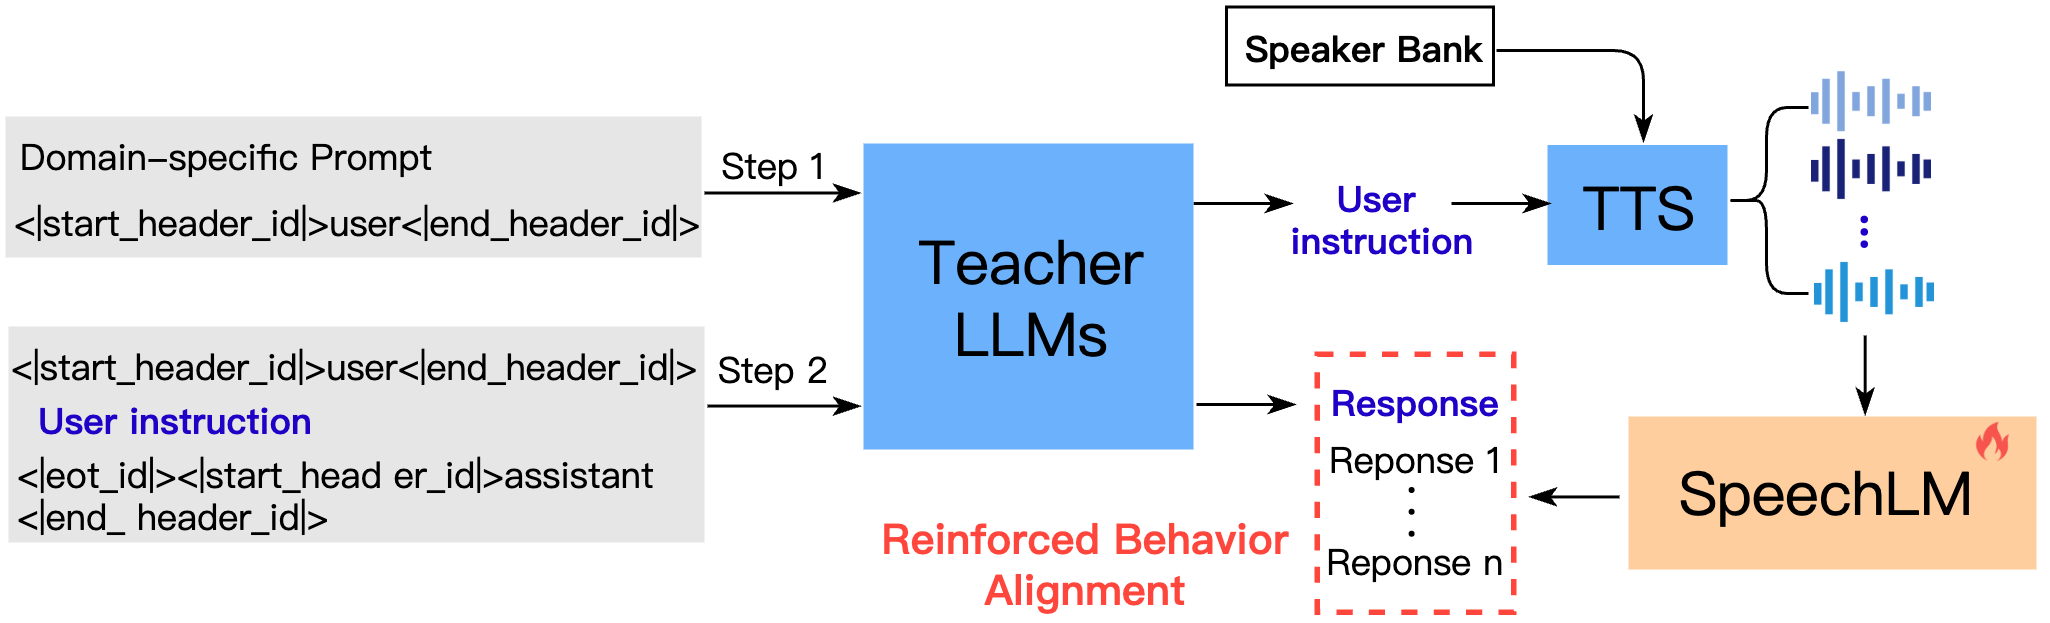
\includegraphics[width=0.98\textwidth]{fig1.jpg}
\end{center}
\caption{Frameworks of RBA. Step 1: generate text user instruction by modifying pre-defined query template, followed by generating spoken instructions by TTS model. Step 2: complete text response by teacher LLMs. }
\label{fig1}
\end{figure*}

\subsection{Self-Synthesis Data Generation}
The initial phase focuses on constructing a comprehensive instruction dataset without relying on human annotations. We leverage a high-capacity aligned LLM (specifically, Llama-3.1-70B-Instruct\footnote{https://huggingface.co/meta-llama/Llama-3.1-70B-Instruct}) as our teacher model to generate both instruction and corresponding response as in Figure~\ref{fig1}. For an aligned LLM, the input sequence can be represented as $x = T_{pre-query} \oplus q \oplus T_{post-query}$. Here, $q$ is the user query (e.g., "Can you introduce the history of pyramid?"), while $T_{pre-query}$ and $T_{post-query}$ are pre-query and post-query templates. As shown in Figure~\ref{fig1}, the $T_{pre-query}$ is set as $\texttt{<|start\_header\_id|>user<|end\_header\_id|>}$, and the $T_{post-query}$ is further annotated by $\texttt{<|eot\_id|>}$. They are both designed to ensure the correct prompting. \par
\noindent \textbf{Instruction Sampling.} The objective of this step is to generate diverse instructions that leverage the extensive pre-training knowledge embedded within LLMs. To this end, we craft a pre-query template that conforms to the predefined instruction format of the teacher LLM. Since LLMs acquire knowledge through autoregressive learning from instruction data during their SFT phase, when presented with our crafted pre-query template, the LLM autonomously generates instructions without requiring any seed questions, thereby ensuring the diversity of generated instructions. Generation continues until the model produces an end-of-sequence token, ensuring complete instruction formation. By repeating this process multiple times, we obtain a large-scale instruction corpus that reflects the knowledge distribution captured during the teacher LLM's training.\par
\noindent \textbf{Response Completion.} Subsequently, the teacher LLM generates corresponding responses to the instructions produced in Step 1. Given that the teacher LLM has undergone SFT and post-training alignment, the resulting instruction-response pairs typically exhibit high quality and behavioral consistency with human preferences. We implement a \textit{filtering} strategy to ensure the suitability of the generated data for speech-based interactions. Specifically, we exclude instructions that are excessively lengthy or involve complex mathematical computations. This filtering criterion is motivated by practical considerations: users rarely pose such technical queries through speech modality due to the inherent difficulty in verbalizing complex mathematical expressions or lengthy technical specifications. By removing these categories, we ensure that our training data better reflects realistic speech-based interaction patterns, where users typically engage with more conversational and direct queries rather than highly technical or verbose instructions. \par
\noindent \textbf{User Speech Generation.} To simulate diverse user speech patterns, we employ the pre-trained CosyVoice TTS system~\cite{du2024cosyvoice} for multi-speaker instruction generation. Our implementation follows three key steps: (1) Speaker Bank Construction.
We leverage the LibriTTS dataset~\cite{zen2019libritts} to create a speaker repository containing 2,456 distinct voices. Each speaker provides a unique vocal fingerprint while maintaining professional-grade articulation. (2) Reference Selection: Utterances exceeding 3 seconds in duration are selected as reference prompts for zero-shot synthesis. This duration threshold ensures sufficient acoustic information for stable voice cloning~\cite{wang2023neural}. (3) Each textual instruction generates 4 distinct spoken sampled from speaker bank, exponentially increasing the SpeechLM's exposure to vocal variations. While LibriTTS speakers exhibit relatively neutral prosody, this characteristic ensures clear enunciation for instruction clarity. Totally, 1 million of samples are generated. \par
\noindent \textbf{Data Analysis.} We use LlaMa-3-8B-Instruct\footnote{https://huggingface.co/meta-llama/Llama-3.1-8B-Instruct} to categorize the generated topic, as shown in Table~\ref{t1}. The predominant topic is "information seeking" with a proportion of 60.3\%, followed by "advice seeking" and "creative writing". This distribution approximately aligns with practical request from human users~\cite{li2023alpacaeval}. To characterize our instruction dataset's complexity distribution, we employ the same model as a difficulty rater. The model assesses each instruction on a 5-level scale ('very easy' to 'very hard') through chain-of-thought reasoning. Our filtered dataset exhibits the following distribution: [26.1\%, 39.2\%, 28.7\%, 52\%, 0.8\%].\par
\noindent \textbf{Discussion on Teacher Model Selection.} While multi-teacher distillation frameworks have demonstrated potential in some scenarios, multiple teachers may introduce conflicting guidance signals (e.g., divergent reasoning patterns) that complicate behavior alignment, particularly detrimental for speech-based tasks requiring stable acoustic-textual mapping. Future work could explore hybrid approaches combining our reinforcement framework with curated multi-teacher knowledge.


\begin{table}[t]
\centering
\caption{Topic distribution in RBA Dataset.}
\label{tab:task_distribution}
\begin{tabular}{l| c }
\toprule
\textbf{Topic Category} & \textbf{Percentage (\%)} \\
\midrule
Information Seeking & 60.3  \\
Advice Seeking & 18.5 \\
Creative Writing & 12.7  \\
Planning & 4.2  \\
Reasoning  & 2.8 \\
Brainstorming & 0.2\\
Role Playing & 0.1 \\
Others & 1.2 \\
\midrule
\textbf{Total} & \textbf{100.0} \\
\bottomrule
\end{tabular}
\label{t1}
\end{table}


\subsection{Reinforcement Learning for SpeechLMs}
Given a speech instruction $x^{(s)}$ from speaker $s \in \{1,2,3,4\}$, the SpeechLM $\pi_{\theta}$ predicts response tokens $y^{(s)} = (y_1^{(s)},...,y_T^{(s)})$. We minimize the cross-entropy loss between predictions and reference responses $y_\mathrm{ref}$:
\begin{equation}
    \mathcal{L}_\mathrm{CE} = -\frac{1}{4}\sum_{s=1}^4 \sum_{t=1}^T \log p_\theta(y_{\mathrm{ref},t} | x^{(s)}, y_{\mathrm{ref},<t})
\end{equation}
Consequently, the SpeeechLM is anticipated to generate responses that closely resemble those from data distribution $(y|x^{(s)})$. However, since the entire SFT process employs teacher-forcing – where SpeechLM predicts the current token based on the reference sequence $y_\mathrm{ref}$ – this creates a discrepancy between training and inference. During inference, the model must rely on its own generated sequence for the first time, leading to the exposure bias problem. RL-based fine-tuning effectively mitigates this issue by optimizing sequences generated through model self-sampling, transforming the supervision signal from SFT's "rote memorization" to encouraging the model to explore and produce higher-quality sequences. \par

\noindent \textbf{Reward Modeling.} 
Given candidate responses $\{y^{(1)},...,y^{(s)}\}$ generated by SpeechLM for spoken instruction, we employ a pre-trained reward model\footnote{https://huggingface.co/RLHFlow/ArmoRM-Llama3-8B-v0.1} to evaluate SpeechLM's responses, where a group of reward $R = \{r^{(1)},...,r^{(s)}\}$ is provided in an online mode. For preference data construction, we propose two distinct positive-negative sampling strategies as follows. \par
\noindent \textbf{RBA-Group}: Within each generated sample group containing multi-speaker inputs, the positive example is selected as the $y^{(s)}$ with highest reward. Despite inherent speaker variations in audio inputs, we enforce speaker-invariant response generation through DPO-based optimization:
\begin{align}
\mathcal{L}_G &= -\log\sigma(\beta\log V^+ - \beta\log  V^-) \\ 
V_{\text{ref}} &= \frac{\pi_{\theta}(y^{(s^+)}|x^{(s^+)})}{\pi_\mathrm{ref}(y^{(s^+)}|x^{(s^+)})}, \ s^+ = \text{arg max} R \\
V^- &= \frac{\pi_{\theta}(y^{(s^-)}|x^{(s^-)})}{\pi_\mathrm{ref}(y^{(s^-)}|x^{(s^-)})}, \ s^- = \text{arg min} R 
\end{align}
where $\pi_\mathrm{ref}$ is the reference model to stabilize the optimization. Empirically, we observe that explicit reference model parameterization can be omitted by directly utilizing reference responses $y_\mathrm{ref}$ for auxiliary supervision as shown in Eq.(1). Then a weight $\lambda$ is employed to balance the $\mathcal{L}_G$ and $\mathcal{L}_{CE}$:
\begin{equation}
    \mathcal{L} = \mathcal{L}_{G} + \lambda \mathcal{L}_{CE} 
\end{equation}    
\noindent \textbf{RBA-Single}: For each generated sample $y^{(s)}$, the corresponding $y_{\mathrm{ref}}$ from teacher LLMs typically exhibit better quality. Therefore, the reward evaluation process can be skipped by directly treating the reference response as the positive sample, while ${y^{(s)}}$ generated by SpeechLM are used as negative samples:
\begin{align}
\mathcal{L}_S &= -\log\sigma(\beta\log V^+_{\text{ref}} - \beta\log  V^-) \\ 
V^+ &= \frac{\pi_{\theta}(y_{\text{ref}}|x^{(s)})}{\pi_\mathrm{ref}(y_{\text{ref}}|x^{(s)})}, \ s\in \{1,2,3,4\} \\
V^- &= \frac{\pi_{\theta}(y^{(s)}|x^{(s)})}{\pi_\mathrm{ref}(y^{(s)}|x^{(s)})}, \ s\in \{1,2,3,4\}
\end{align}
Although the outputs from SpeechLM are not necessarily always undesired, existing work~\cite{chen2024self} has theoretically verified the feasibility of this approach and demonstrated that it achieves comparable or even superior performance to SFT. 


\subsection{Extension on SQA and S2TT}
Besides instruction-following, we take SQA and S2TT as examples to demonstrate how RBA can substantially enhance the task-specific performance of SpeechLMs. \par
We developed a rapid Q\&A dataset called RBA-QA to enhance SpeechLM's real-world knowledge. A total of 20,000 questions are generated by teacher LLMs and paired with answers. This dataset exhibits two key distinctions from conventional RBA dataset: (1) Single-Speaker Design: Each spoken question is synthesized using only one speaker profile. (2) Concise Answers: Responses are strictly constrained to 1-5 words. During optimization, we exclusively employ the RBA-Single strategy because the baseline SpeechLM often fails to produce valid answers for these questions, making positive sample selection impractical. \par
Given a source language in spoken form, the S2TT task aims to predict the text in the target language. In public datasets, the source language text is usually available, and the teacher LLM generates the reference text prediction based on this transcript. After sampling with SpeechLM, the BLEU score between its output and the reference text is used as the reward to select positive and negative samples for RBA-Group optimization. RBA-Single continues to follow the original setting. In general, this approach does not require supervised labels, and SpeechLM can effectively aligns its behavior with the teacher LLM when only source speech is available. \par
\begin{table*}[t]
\centering
\resizebox{1.00\textwidth}{!}{%
\begin{tabular}{l|c|cc|cc|cc|cc}
\toprule
\multirow{2}{*}{Evaluation Topic} & \multirow{2}{*}{\#Num.} & \multicolumn{2}{c|}{RBA-G v.s. Base.}  & \multicolumn{2}{c|}{RBA-G v.s. Ref.}   & \multicolumn{2}{c|}{RBA-S v.s. Base.}  & \multicolumn{2}{c}{RBA-S v.s. Ref.}   \\    
 & & WR(\%)& LC(\%)  &WR(\%)& LC(\%)  &WR(\%)& LC(\%)  &WR(\%)& LC(\%) \\ \midrule    
\textit{Information Seeking} & 603k & 79.5 & 55.0 & 42.0 & 47.5 & 95.0 & 76.5 & 46.5 & 48.0 \\
\textit{Advice Seeking} & 185k & 77.0 & 56.5 & 41.0 & 44.5 & 85.5 & 72.5 & 40.5 & 44.0 \\
\textit{Creative Writing} & 127k & 74.5 & 60.0 & 46.5 & 45.5 & 89.0 & 70.0 & 48.5 & 46.0 \\
\textit{Planning} & 42k & 72.5 & 61.0 & 45.0 & 45.5 & 88.0 & 80.0 & 47.5 & 44.0 \\
\textit{Reasoning} & 28k & 81.0 & 55.5 & 40.5 & 41.0 & 95.5 & 70.5 & 43.0 & 44.5 \\
\textit{Brainstorming} & 2k & 73.0 & 71.0 & 44.0 & 45.5 & 89.0 & 73.5 & 45.0 & 46.0 \\
\textit{Role Playing} & 1k & 72.0 & 66.5 & 39.0 & 43.0 & 78.5 & 73.5 & 41.0 & 43.5 \\
\textit{Others} & 12k & 73.5 & 65.5 & 41.0 & 42.0 & 79.0 & 70.0 & 42.0 & 43.5 \\
\midrule
\textit{Spoken-Alpaca} & N.a. & 65.5 & 60.5 & 43.0 & 39.5 & 74.0 & 63.0 & 44.5 & 46.0 \\
\bottomrule
\end{tabular}}
\caption{Win-Rate (WR) and Length-Controlled Win Rate (LC) results evaluated by GPT-4o. Each topic contains 200 testing examples. "\#Num." is the number of training example of each category. "Base." and "Ref." denote the generated response by Qwen-audio2 and LLaMA3-70B, which can be viewed as baseline and upper bound of RBA.}
\label{tab1}
\end{table*}
\begin{table}[]
\centering
\resizebox{0.49\textwidth}{!}{%
\begin{tabular}{c|ccc}
\toprule
Model &  Web-Q & Llama-Q & TriviaQA \\ \midrule
GSLM~\cite{lakhotia2021generative}  & 1.5 & 4.0 & -   \\ 
TWIST~\cite{hassid2023textually}  & 1.1 & 0.5 &   \\ 
SpeechGPT~\cite{zhang2023speechgpt}  & 6.5 & 21.6 & 14.8   \\ 
Spectron~\cite{nachmani2023spoken}  & 6.1 & 21.9 & -   \\ 
Moshi~\cite{defossez2024moshi} &  26.6 & 62.3& 22.8   \\ 
GLM-voice~\cite{zeng2024scaling} &  32.2 & 64.7 & 39.1   \\ \midrule
Baseline Model &10.1 & 33.4 & 19.7\\ 
BRA-S &  \textbf{40.7} & \textbf{77.0} &  \textbf{55.1} \\
\bottomrule
\end{tabular}}
\caption{Accuracy (\%) results on SQA task, where RBA-S is compared with other competitive models.}
\label{table2}
\end{table}
\begin{table*}[h]
\centering \resizebox{0.96\textwidth}{!}{%
\begin{tabular}{p{0.24\linewidth}|p{0.7\linewidth}}
\toprule
\textbf{Response by} & \textbf{User Input}: Propose an ethical solution to the problem of data privacy. \\
\midrule
SpeechLM (\textit{before} RBA) & 
Rely on user agreements and opt-in consent mechanisms. By clearly informing users and letting them choose whether or not to share data, the solution respects autonomy. However, it may be insufficient in practice due to information asymmetry and low user engagement. (GPT score: \textbf{6.0})\\
\midrule
SpeechLM (\textit{after} RBA)& 
Use data minimization and purpose limitation principles: collect only the data strictly necessary for a task and ensure it is not repurposed without user consent. This approach is simpler than differential privacy but still supports ethical handling of personal data. (GPT score: \textbf{8.0}) \\
\midrule
Teacher LLM & Implement differential privacy across all data collection and processing pipelines. This mathematical framework ensures that individual user data cannot be reverse-engineered from aggregate outputs, even by internal actors. Combined with strict access control and transparency reporting, this provides a high standard for ethical data privacy. (GPT score: \textbf{9.5})\\
\bottomrule
\end{tabular} }
\caption{Responses from different models and their GPT scores. The user input is from \textit{Spoken-Alpaca} dataset. For SpeechLM, the input is in spoken formats while the teacher LLM consumes text.}
\label{case}
\end{table*}
\section{Experimental Setting}
\subsection{Dataset and Metric}
For the RBA dataset, we select 200 samples from each topic category to construct a test set, totaling 1,600 samples. To validate the generalization capability of our method, we sample 200 out-domain questions from the Spoken-Alpaca dataset (GSQA/spoken-alpaca-gpt4) as an out-of-domain test set. Furthermore, Web-Questions~\cite{berant2013semantic}, Llama-Questions~\cite{nachmani2023spoken}, and TriviaQA~\cite{joshi2017triviaqa} are employed to demonstrate improvements in real-world knowledge comprehension.  
Our primary experiments utilize Qwen2-Audio~\cite{chu2024qwen2} (8B) as the SpeechLM backbone, where its performance is viewed as baseline. To verify the efficacy of RBA, we adopt the following evaluation metrics from GPT-4o (2024-08-06):
\begin{itemize}
    \item Win-Rate (\textbf{WR}): the fraction of responses that are favored by the GPT evaluator.
    \item Length-Controlled Win Rate (\textbf{LC}): a debiased version of WR from~\cite{dubois2404length} 
    \item Accuracy (\textbf{Acc}): the correct rate of responses. 
\end{itemize}
For S2TT, we select the source language from FLEURS~\cite{conneau2023fleurs}, CoVoST2~\cite{wang2021covost}, and MuST-C~\cite{di2019must}, resulting in 327K X$\rightarrow$En and En$\rightarrow$X pairs. Their training set is employed for training while the original test sets with labels are used for evaluation in terms of BLEU score. 
\subsection{Training Details}
During the data generation phase, we configure the teacher LLM with temperature settings ranging from 1.0 to 1.2 and Top-P values between 0.99 and 1.00 to encourage the diversity. The computational infrastructure utilizes 128 NVIDIA A100 (80GB) GPUs for and 64 A40 (48GB) GPUs for data synthesis and model training.

The learning rate follows a 3,000-step warmup schedule to achieve max value of 1e-4, the weight decay is set as 0.98. For validation, we randomly select 128 data points from each domain to construct validation sets, which guide checkpoint selection and early stopping criteria. Hyperparameters are configured with $\lambda$ = 0.2 and $\beta$ = 0.1 to balance alignment strength and distribution preservation. In practice, both hyper-parameters are not sensitive to experimental results.

\section{Result}
In this section, we design experiments to address the following questions and demonstrate the efficacy of RBA approach: (1) Does RBA enhance general instruction-following capabilities of SpeechLM across different topics and external evaluation set? (2) Does RBA improve SpeechLM's factual knowledge and lead other models in SQA accuracy? (3) How does the RBA-enhanced model perform on S2TT capability with unlabeled speech, and can it compete with task-specific models? (4) Does our proposed reinforcement learning optimization strategy outperform SFT?
\subsection{Result on Instruction-Following}


\begin{table}[]
\centering
\resizebox{0.47\textwidth}{!}{%
\begin{tabular}{l|cc|cccc}
\toprule
\multirow{2}{*}{Test Set}& \multicolumn{2}{c|}{RBA-G v.s. SFT}  & \multicolumn{2}{c}{RBA-S v.s. SFT}   \\    
 &  WR(\%)& LC(\%) & WR(\%)& LC(\%) \\ \midrule    
 In-domain  & 52.7 & 50.6 &  56.0 & 51.3\\ \midrule    
 Out-domain & 55.0 & 52.6 &  57.1 & 53.4   \\ \bottomrule
\end{tabular}}
\caption{``SFT" is the model that learns from teacher LLM's generations using the cross-entroy loss in Eq.(1).}
\label{sft}
\end{table}
\begin{table*}[t]
\centering
\resizebox{1.00\textwidth}{!}{%
\begin{tabular}{c|ccccccccccccccc|c}
\toprule
Model (X$\rightarrow$En) &Ar &Cy & De &El &Es& Fa& Fr& Hi& It& Ja& Pt& Ta& Uk& Vi& Zh& Avg. \\  \midrule 
Whisper-large V2& 25.5 & 13.0 &34.6 & 23.7 &23.3 &19.6 &32.2 &22.0  &23.6 &18.9 &38.1& 9.2& 29.4 &20.4& 18.4& 23.5 \\
SeamlessM4T-L & 32.8 & 31.7 &35.8 &25.6 &25.0 &28.2 &33.1 &26.3 &25.0 &17.0 &38.9 &16.0 &30.2 &21.6 &19.8 &27.1 \\
AudioPaLM2 & 29.0 &7.2 &38.7& 18.8& 26.9& 25.7& 36.5 &21.7 &27.8 &11.1 &38.4 &15.0 &26.9 &15.6 &21.3 &24.0 \\ 
SeamlessM4T-L V2& 34.7 &34.9 &37.1 &27.3 &25.4 &30.3 &33.7 &28.5 &26.5 &19.5 &38.5 &22.1 &33.2 &25.7 &23.0& 29.4 \\ \midrule
RBA-S & 35.1 & \textbf{36.8} & 37.3 & 25.2 & 40.1 & 36.1 & \textbf{34.4} & 31.6 &  37.1 & \textbf{19.9} & \textbf{39.1} & 26.2 & 31.3 & 27.9 & 30.0 & 32.5  \\
RBA-G & \textbf{36.3} & 36.1 & \textbf{37.6}& \textbf{26.9} & \textbf{40.3} & \textbf{36.9} & \textbf{34.4} & \textbf{32.7} &\textbf{39.7}& 17.7   & 38.2 & \textbf{28.0} & \textbf{33.6} & \textbf{28.8} & \textbf{30.8} & \textbf{33.2}  \\
\bottomrule
\end{tabular}}
\caption{BLEU results of S2TT task (X$\rightarrow$En) on FLEURS benchmark.}
\label{table6}
\end{table*}



To evaluate whether RBA improves SpeechLM's instruction-following performance, we conduct comprehensive experiments across multiple domains and assess generalization on external datasets in Table~\ref{tab1}. It is observed that both RBA variants substantially improve SpeechLM's instruction-following capabilities, with RBA-Single consistently outperforming RBA-Group across all evaluated domains. \par

\noindent \textbf{RBA v.s. Baseline}. For in-domain performance, RBA-S achieves win rates of 78.7\%-95.5\% against the baseline, with particularly strong performance on Information Seeking (95.1\%) and Reasoning (95.5\%) tasks. RBA-G shows more modest improvements, ranging from 71.8\%-80.8\% win rates. On the out-of-domain Spoken-Alpaca dataset, RBA-S maintains strong performance (74.1\% win rate vs. baseline), demonstrating robust cross-domain transfer. RBA-G shows reduced but still significant improvement (65.5\% win rate), indicating that both methods generalize beyond training domains. An case study is visualized in Table~\ref{case} for comparison. After RBA, the generation quality is obviously improved, supported by GPT score.  \par
\noindent \textbf{RBA v.s. Reference}. When compared against teacher LLM references, both variants achieve 40-48\% win rates across different domains, representing substantial progress toward teacher-level performance despite processing various speech inputs rather than clean text. \par
\noindent \textbf{RBA-G v.s. RBA-S}. RBA-Single consistently outperforms RBA-Group by 6-15 percentage points across all domains, though the former eliminates the reward evaluation process. This performance gap suggests that: (1) Due to the teacher LLM's significant performance advantage over SpeechLM, its generated responses inherently exhibit superior quality. This inherent quality gap allows reward modeling to be partially omitted in practice. (2) RBA-S demonstrates better sampling efficiency by fully utilizing every generated sample, whereas group-based approaches like RBA-G discard potentially useful intermediate-quality samples. (3) RBA-G faces inherent limitations where an entire speaker group might fail to explore high-quality samples (e.g., all four speaker versions generating suboptimal responses), thereby constraining its maximum achievable performance. \par
\noindent \textbf{RBA v.s. SFT.} We demonstrate the superiority of reinforcement learning-based optimization over SFT by comparing RBA-generated outputs with SFT results. As shown in the tables~\ref{sft}, both RBA-Group and RBA-Single exhibit advantages over baselines across in-domain and out-of-domain evaluations. This validates the effectiveness of using self-sampled training data for model alignment, which aligns with recent findings in instruction tuning literature~\cite{chen2024self}.

\

\begin{table}[]
\centering
\resizebox{0.42\textwidth}{!}{%
\begin{tabular}{c|cccccc}
\toprule
\multirow{2}{*}{Model} &\multicolumn{6}{c}{En $\rightarrow$ X}\\
  &  De & Zn &Es & Fr & It& Avg.\\
\midrule
Base.& 25.9 & 45.2 & 21.4 &  37.1 & 22.0 & 30.3 \\ 
SFT & 26.0 & 45.0 & 21.4 & 37.4 & 22.7 & 30.5\\
RBA-S & 27.7 & 46.0 & \textbf{26.2} &35.9 & \textbf{27.0} & 32.6\\
RBA-G & \textbf{30.3} & \textbf{47.3} & 23.8 & \textbf{38.1} & 25.1 & \textbf{33.0} \\ \midrule
Ref. & 36.0 & 49.7 & 33.6 & 47.7 & 34.4  &40.3\\
% RBA-S   & 40.1 & 34.4 & 37.1 \\
% RBA-G   & \textbf{40.3} & 34.4 & \textbf{39.7} \\
\bottomrule
\end{tabular}}
\caption{BLEU results (En $\rightarrow$ X) on CoVoST-2.}
\label{table5}
\end{table}

\subsection{Result on SQA}
The accuracy result of SQA task is reported in Table~\ref{table2}. Given that the RBA-QA dataset contains only single-speaker samples, we exclusively employed the RBA-Single optimization strategy. The RBA-QA data was combined with the original training set and fine-tuned for 2 additional epochs to prevent catastrophic forgetting while incorporating new knowledge. We observe that RBA successfully enhances SpeechLM's factual knowledge comprehension and establishes new state-of-the-art results on standard SQA benchmarks, confirming its effectiveness for knowledge-intensive spoken language understanding tasks.




\subsection{Result on S2TT}

We first report the En $\rightarrow$ X translation results in Table~\ref{table5}. SFT achieves only marginal gains over the baseline model (30.5 vs. 30.3 average BLEU), representing a mere 0.2-point improvement. This limited effectiveness stems from SFT's fundamental approach of fitting the model to a new distribution without adequately addressing the modality gap between speech and text representations. Contrary to instruction-following tasks, RBA-G achieves superior performance (33.0 average BLEU) compared to RBA-S (32.6 average BLEU). This reversal occurs because: (1) Quality of SpeechLM Translation Samples: The SpeechLM inherently generates reasonable translation outputs, providing a solid foundation for group-based optimization. (2) Self-Generated Sample Exploration: RBA-G leverages purely self-generated training samples to explore superior translation strategies through contrastive learning across speaker variations. Despite significant improvements, both RBA variants maintain substantial gaps compared to references. \par

Then the X$\rightarrow$En translation with other competitive models are report in Table~\ref{table6}. The 3.8 BLEU improvement over SeamlessM4T-Large V2 is particularly significant, given that SeamlessM4T is specifically designed and optimized for multilingual translation tasks. The results validate RBA's contribution that effective behavioral alignment can enable general-purpose SpeechLMs to match or exceed specialized architectures without task-specific engineering. This finding is particularly impressive given that competing models (Whisper~\cite{radford2023robust}, SeamlessM4T~\cite{barrault2023seamlessm4t}, AudioPaLM~\cite{rubenstein2023audiopalm}) are explicitly optimized for translation tasks, while RBA maintains its instruction-following capabilities. 

\subsection{Analysis of Cross-Speaker Output Consistency}
A critical question arises from our methodology: since both the SFT baseline and the RBA-G model are trained on the same multi-speaker data, what is the precise source of RBA's enhanced robustness? We posit that the key difference lies not in the data exposure itself, but in the fundamental nature of the optimization objective. This experiment is therefore designed to empirically validate that RBA-G's intra-group contrastive learning, rather than SFT's independent supervision, is the primary driver of speaker-invariant behavior.

To test this hypothesis, we conducted an output consistency analysis. The premise is that a truly robust model should produce semantically consistent responses to the same instruction, regardless of which speaker's voice is used for the spoken input. We sampled 500 instructions from our in-domain test set and fed their four corresponding spoken versions (each from a different speaker) into both our final RBA-G model and the SFT baseline. This process generated a group of four responses per model for each instruction. We then quantified model stability by measuring the Average Pairwise Semantic Similarity within each group of four responses, using a pre-trained sentence-transformer (paraphrase-mpnet-base-v2) to compute cosine similarity.  \par
\begin{table}[h]
\centering
\resizebox{0.36\textwidth}{!}{%
\begin{tabular}{l|c}
\toprule
\textbf{Model} & \textbf{Output Consistency Score (↑)} \\
\midrule
Baseline & 0.826\\
SFT & 0.893 \\
RBA-G  & \textbf{0.945} \\
\bottomrule
\end{tabular}%
}
\caption{Cross-speaker output consistency results. The score measures the average semantic similarity of a model's responses to the same instruction spoken by four different speakers. A higher score indicates greater robustness to acoustic variations.}
\label{table_consistency_final}
\end{table}
The results in Table~\ref{table_consistency_final} provide direct evidence supporting our hypothesis. The RBA-G model achieves a remarkably high consistency score of 0.945, confirming that its outputs are semantically stable across different speaker inputs. In contrast, the SFT model scores significantly lower at 0.893. This variability persists despite SFT being trained on all four speakers because the standard cross-entropy loss treats each pair as an independent sample; it lacks an explicit mechanism to enforce consistency across the samples within an instruction group. RBA-G's superior consistency stems from its inherently relational objective. By rewarding the best response and penalizing the worst from within the group of self-generated samples, it creates a powerful optimization pressure for the model to converge on a single, robust policy that performs well for all speakers.


\section{Conclusion}
In this paper, we explore how to leverage a teacher LLM to enhance the reasoning and knowledge capabilities of SpeechLMs. To this end, we construct a knowledge transfer dataset via a self-synthesis approach, and propose a reinforcement learning-based alignment method to effectively bridge the modality gap. Experimental results demonstrate significant improvements in both instruction-following ability and factual knowledge acquisition. Moreover, we show that the proposed method can be seamlessly extended to S2TT tasks, achieving competitive performance on public benchmarks without relying on any labeled data.





\bigskip
\newpage

\bibliography{aaai2026}

\end{document}
